\documentclass[journal]{IEEEtran}
\usepackage{graphicx}
\usepackage{tikz}
\usepackage{mathtools, amsfonts, breqn, subcaption}
\DeclareMathOperator*{\argmin}{arg\,min}
\begin{document}

\title{Experimental Evaluation of Control Policies for \\Segway Robot in Dynamic Environments }
\author{Ian~Buckley, Niharika~Arora, Varun~Murali}
\markboth{ECE6552, 26 April 2016}%xdf
{Shell \MakeLowercase{\textit{et al.}}: Project Proposal}
\maketitle
%%%%%%%%%%%%%%%%%%%%%%%%%%%%%%%%%%%%%%%%%%%%%%%%%%%%%%%%%%%%%%%%%%%%%%%%%%%%%%%%%%%%%%%%%%%%%%%

\begin{abstract}
Successful navigation, which involves moving from one location to another while avoiding collisions with obstacles in the environment, is a fundamental objective for mobile robots. A combination of deliberative and reactive control allows mobile robots to achieve planned navigation while avoiding unexpected obstacles or deviations from the plan. A hybrid approach, inspired by nonlinear control and enabled by barrier functions, is proposed. Using quadratic programming to determine inputs simultaneously satisfying control constraints from control Lyapunov and barrier functions, this paper presents a nonlinear navigation control protocol. Motivation and explanation of the protocol are presented. Verification of the navigation control protocol is performed first in MATLAB simulation, which shows that the control law correctly drives the robot first to a target location and second to a trajectory generated using a probabilistic roadmap algorithm. After verification in simulation, the navigation control protocol is implemented on a real robotic system, demonstrating that the nonlinear navigation control protocol successfully traverses the gap between theory and practice. 
\end{abstract}

\section{Introduction}
Navigation is of fundamental concern for mobile robots. The ability to successfully avoid obstacles, both static and dynamic, while moving towards a goal location largely determines the utility of a mobile robotic platform. It is critical that robots avoid obstacles for their own safety as well as the safety of the people around them. Given the importance of navigation, it is not surprising that the problem has long been considered and explored; furthermore, it is reasonable to assert that approaches to the problem are as varied as the disciplines related to robotics themselves.  

Both deliberative and reactive approaches to navigation have been explored. Deliberative approaches navigation benefit from optimal path planning, but suffer when reality deviates from the map, either due to mapping inaccuracies or dynamic obstacles. Probabilistic roadmaps for path planning, first presented by Kavraki et. al. in \cite{kavraki1996}, are a deliberative approach to navigation in which a search algorithm is applied to a map in order to identify a possible path through the environment. In contrast, reactive approaches to navigation may not find optimal solutions and are susceptible to local minima but are able to respond to dynamic obstacles and the environment as it is encountered. Artificial potential fields are a reactive method of navigation that have long been considered~\cite{khatib1985}. Hybrid approaches to navigation take planning and layer it with reactive controls that handle possible obstacles.

%TODO citations needed towards the end
Nonlinear control based navigation is also a studied problem such as by Ting et al. \cite{ting2014reactive}. Generating a policy in a reactive fashion reduces the complexity of the computation needed. Traditional path planners can be used to provide a high level trajectory by having some previous metric knowledge of the space. Lower level reactive controllers can be used for local refinement of the global path and can be used to control the robot--this reduces the complexity of re-planning every time a change in the environment is observed. Potential field based algorithms have been used to generate such reactive policies in the past with some success. There are some known pitfalls for this method with regards to local minima but several solutions for this have been proposed.

Given the possibility of having a global metric representation of a domestic environment, a global trajectory can be generated and a local non-linear controller that obeys constraints imposed by the robot and the objective could be used to achieve navigational objectives. In this paper, control Lyapunov and barrier functions are designed for robot navigation and collision avoidance. Constraints important for navigation, such as distance from obstacles, distance to target, deviation from desired heading, minimum and maximum velocity, and minimum and maximum rotational velocity will be combined to generate a navigation control protocol for the robot. Quadratic programming as presented by Ames et. al. in \cite{amesACC} will be used to simultaneously satisfy these constraints. Furthermore, by applying nonlinear control to navigation, claims about stabilization of the robot to the navigational directive can be guaranteed theoretically, which is an improvement over other reactive navigation methods, which can make no such claims.

The navigation control protocol will first be motivated and derived. After explaining the protocol, MATLAB simulation will be used to verify that the navigation control protocol correctly drives the state of the robot to a target. After demonstrating that the robot can navigate to a target location, a trajectory will be generated for a map using a probabilistic roadmap, and the control law will be used to drive the robot along the trajectory. After thoroughly verifying the navigation control protocol in simulation, the controller will be implemented in the ROS framework and evaluated on the mobile robot Jeeves, shown in Figure \ref{fig:jeeves}, which will verify the navigation control protocol in a real world scenario.

\section{System Description and Dynamics}
The robotic system considered in this paper and its dynamics are presented. The dynamics of the system, and thereby the control objectives, must be twice considered. First, the control objective of the robot to remain balanced is a primary objective that is achieved by a low-level control protocol outside the scope of this project. Second is navigation directive, which is achieved through the control protocol presented in this paper. The following sections describe the system and detail the dynamics.
   
\subsection{System Description}
\begin{figure}
    \centering
    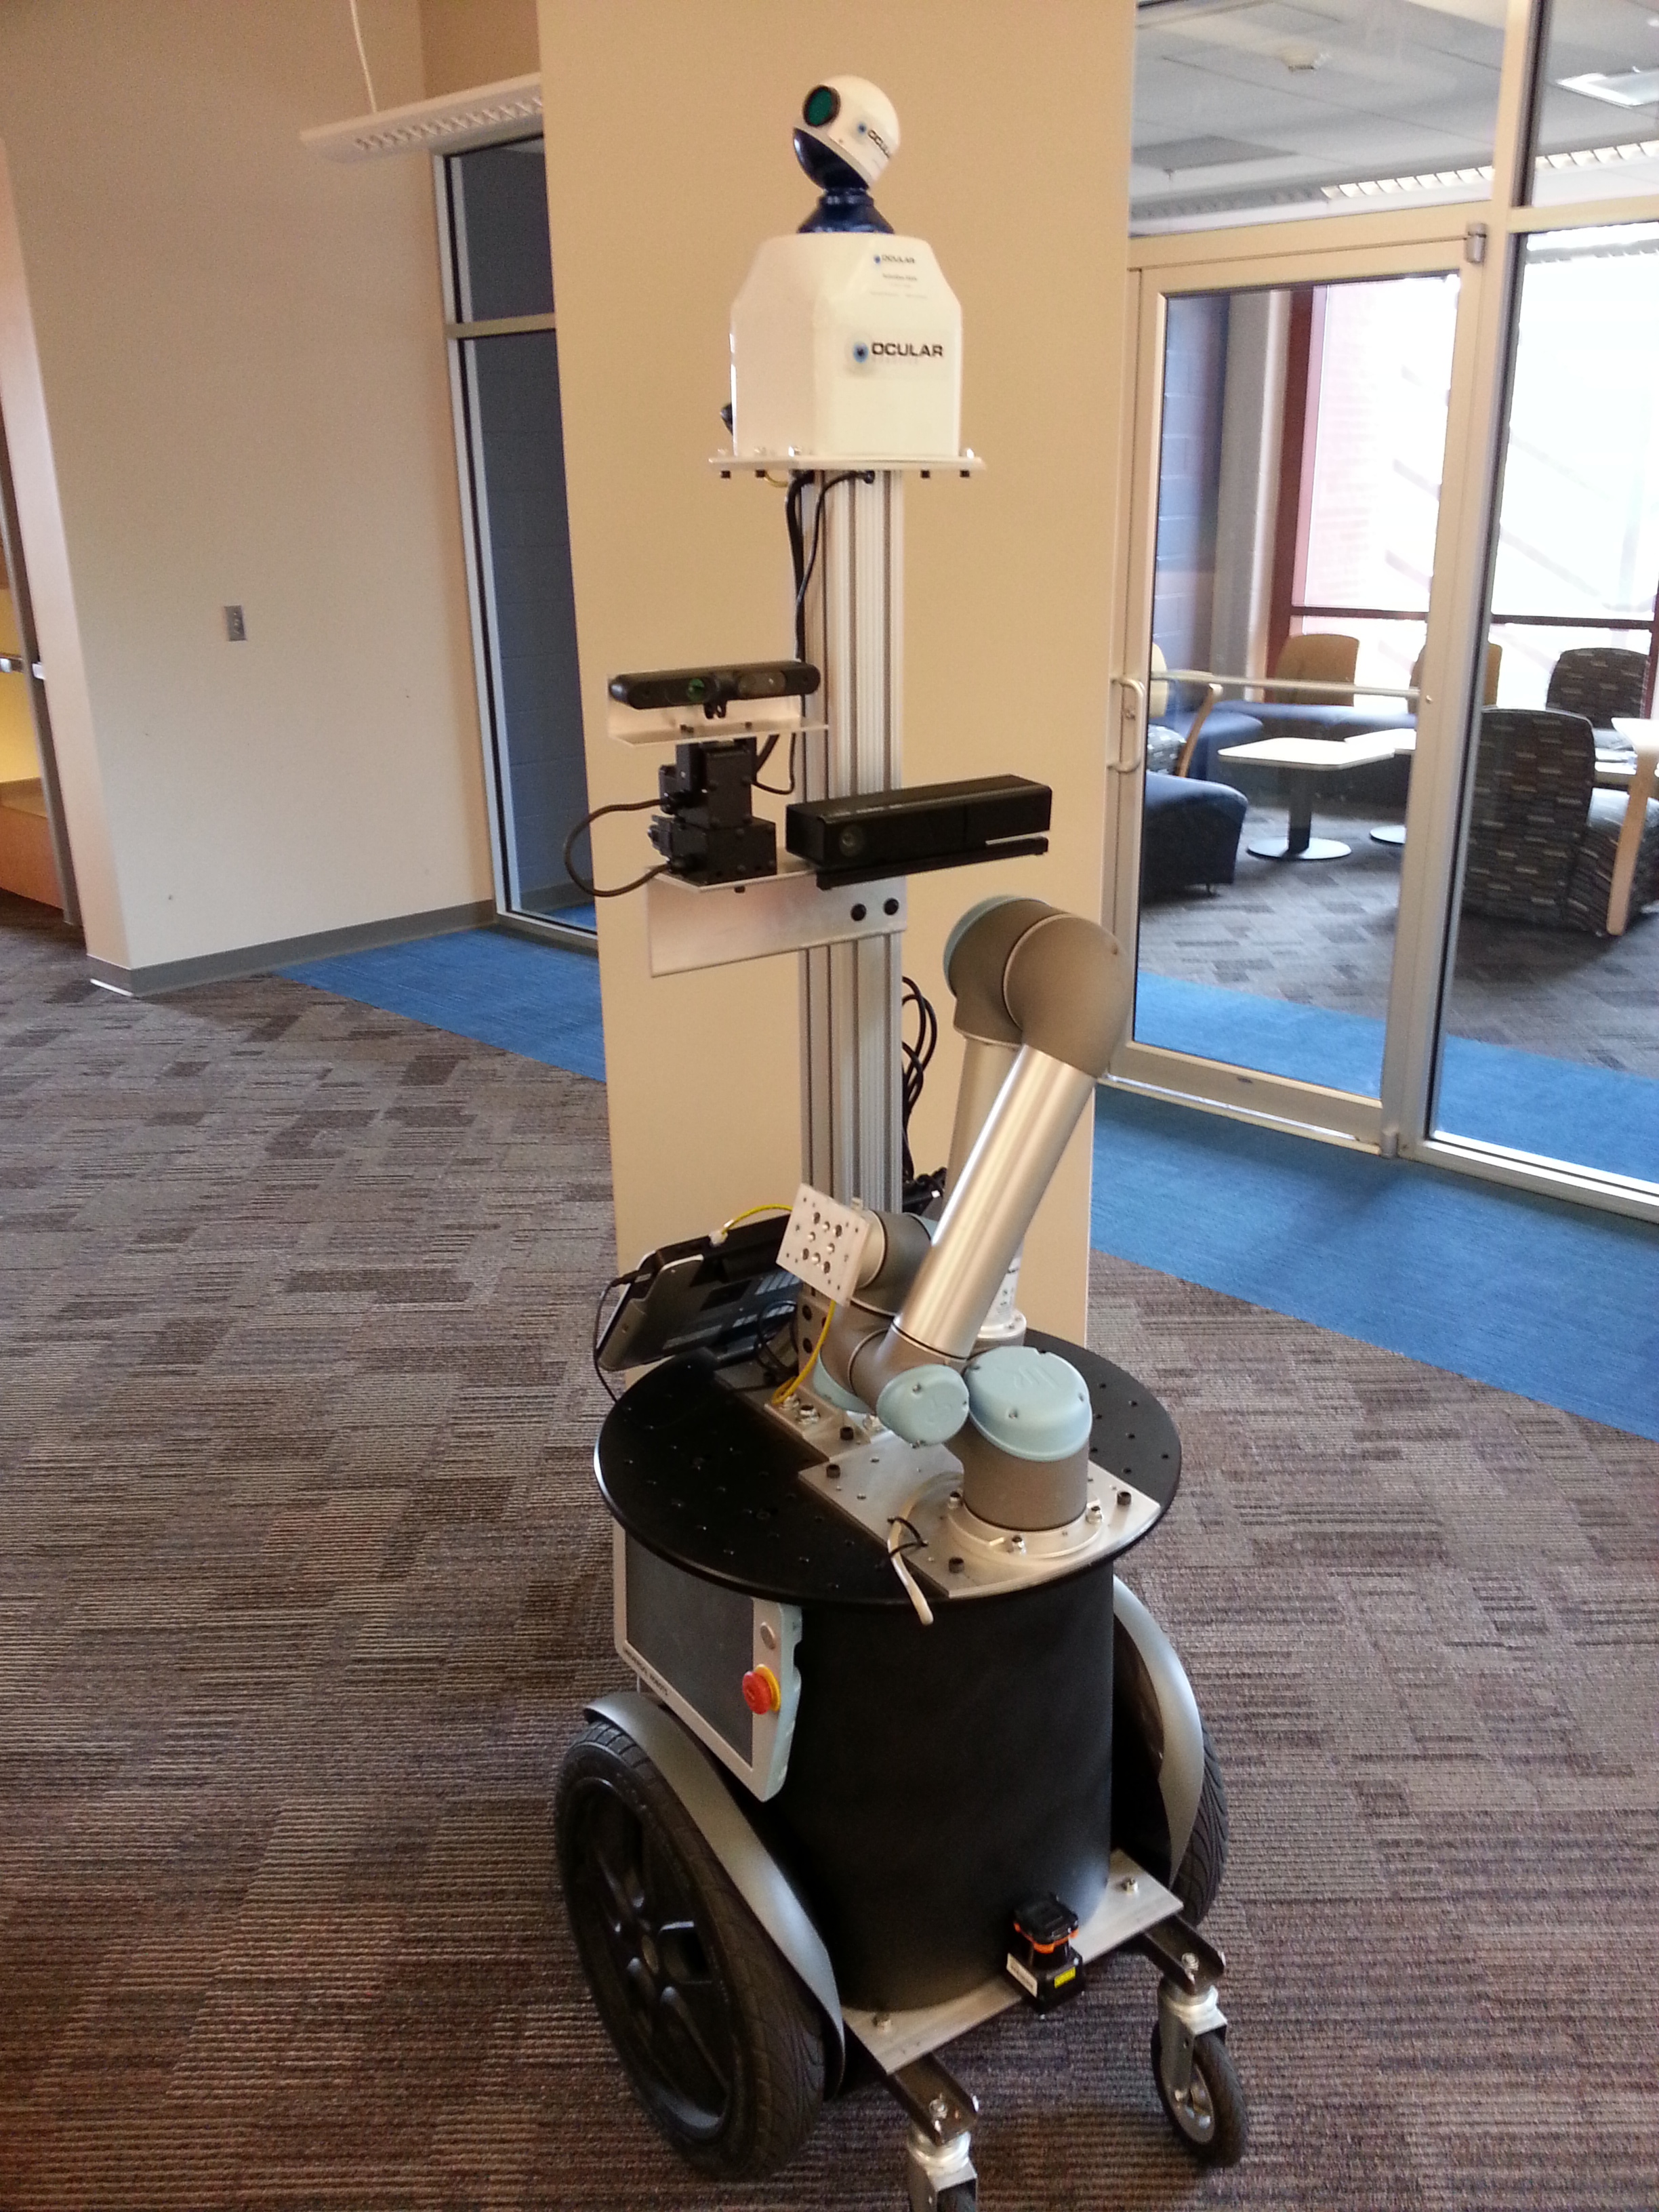
\includegraphics[width = 4cm, scale=0.2]{jeeves2_0.jpg}
    \caption{Jeeves - A modified Segway based robot mounted with a Primesense, Microsfot Kinect, Roboteye RE05, Hokuyo LTM-30x laser and the UR5. Currently modified to include the casters for static stability}
    \label{fig:jeeves}
\end{figure}

\begin{figure}
    \centering
    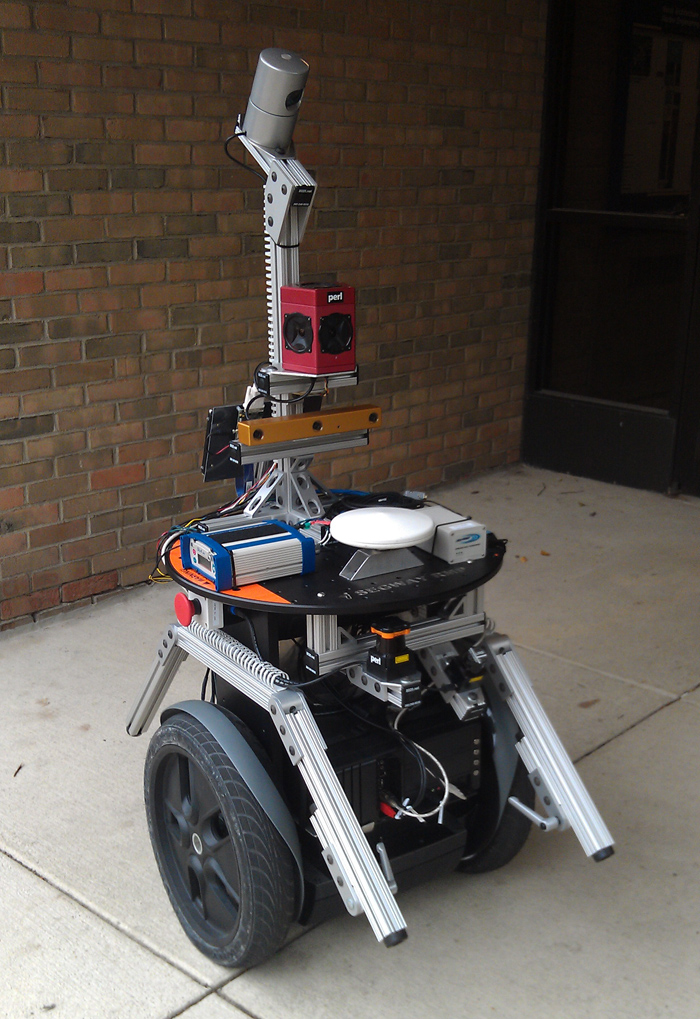
\includegraphics[width = 4cm, scale=0.2]{segway1.jpg}
    \caption{Proposed modification to the Segway base inspired by the Segway robot at the University of Michigan}
    \label{fig:mod_jeeves}
\end{figure}

The robot platform shown in Figure \ref{fig:jeeves} consists of a Segway RMP-200 mobile base, which has been
modified to hold various sensors. The Seqway RMP 200 has been modified to be statically stable but for the purposes of this project, the casters shall be removed and 8020 adjustments will be made on the side of the robot to prevent it from tipping (inspired by Figure \ref{fig:mod_jeeves}). The sensor suite on the robot consists of a Roboteye RE05 sensor capable of scanning in 3D, a primesense RGB-D camera and a Kinect RGB-D. The Hokuyo LTM-30x is mounted at the base and used for base obstacle avoidance. 

In the scope of this project, the Hokuyo LTM-30x is used to detect obstacles from a planar scan. The closest laser hit can be considered an obstacle and dynamic obstacles can be modelled in this way. A microstrain IMU is mounted on the robot to estimate the state of the robot.

The robot is controlled using a PS3 controller when in tele-operation mode, which has a manual override and a dead-man switch to kill the robot due to any type of failure. The robot is also permanently connected to a computer that is monitoring the robot and can be used to kill running programs on the robot.

The control law will further be used to test how it affects the dynamics of the system. We will measure the translation and the rotational velocities and the tip angle to verify that the control policy doesn't force the robot to go beyond its boundary conditions and ensures its safety.

\subsection{Nonlinear Dynamics}
The dynamics (discussed in \cite{castro2012modeling}) of the Segway RMP base can be modelled as a cart with an inverted pendulum which can be modelled as:
\begin{equation}
 mL\text{ sin}(\theta)\dot{\theta}^2 + (M+m)\dot{v} - F - mL\text{ cos}(\theta)\ddot{\theta} = 0, 
\end{equation}
where $\theta$ is the angle of the pendulum with respect to its vertical position, $v$ is the speed of the base, $F$ is the force on the cart, $M$ is the mass of the cart and $m$ is the mass of the pendulum and $L$ is the length of the massless rod. While these dynamics are important, they are handled by a low-level controller and are outside the scope of this project. 

Of greater relevance to navigation, the robot was assumed to be modelled by unicycle dynamics for the purpose of designing the navigation control protocol proposed by this paper. The unicycle dynamics model is presented in the familiar rectangular form:
\begin{equation}
\left(
\begin{matrix}
\dot{x}\\
\dot{y}\\
\dot{\theta}
\end{matrix}
\right)
=
\left(
\begin{matrix}
v \text{ cos}(\theta)\\
v \text{ sin}(\theta)\\
\omega
\end{matrix}
\right),
\end{equation}
where $(x,y)$ are the global coordinates of the robot, and $\theta \in (-\pi ,\pi]$ is the angle formed between the heading of the robot and the positive $x$-axis--$v$ and $w$ are the linear and translational velocities respectively. While control of the unicycle robot is possible using rectangular dynamics, a transformation of the dynamics into polar form simplifies the dynamics for formulating the control law, where $r=\sqrt(x^2+y^2)$ is the distance between the goal and the robot, and $\theta$ is unchanged. The polar coordinates are transformed yet again into an egocentric coordinate system centered on the robot to represent the heading of the robot $\delta$; this transformation was inspired by \cite{park2011}. The final form of the dynamics is given by:  

\begin{figure}[h!]
\begin{center}
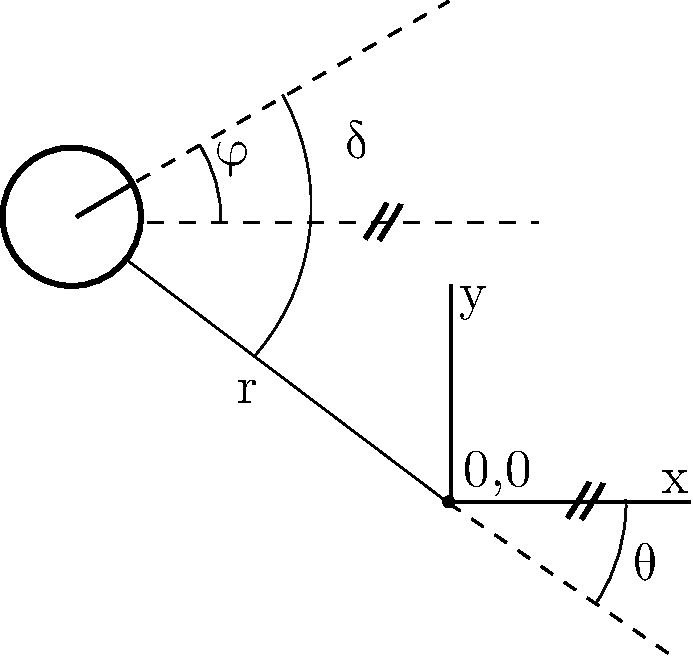
\includegraphics[scale=0.45]{uni.pdf} 
\caption{Egocentric Polar Unicycle Dynamics\label{fig:uni}} 
\end{center}
\end{figure}

\begin{equation}
\left(
\begin{matrix}
\dot{r}\\
\dot{\theta}\\
\end{matrix}
\right)
=
\left(
\begin{matrix}
- v \text{ cos}(\delta)\\
\frac{v}{r} \text{ sin}(\delta)\\
\end{matrix}
\right).
\end{equation}
\begin{equation}
\dot{\delta}=\frac{v}{r} \text{ sin}(\delta)+\omega
\end{equation}

Figure~\ref{fig:uni} describes relationships between the coordinate system used by the dynamics above. The angle $\phi$ is the heading of the robot in the global coordinate frame, $\delta$ is the egocentric heading, $\theta$ is the angle that the robot frame makes with the positive $x$-axis in global coordinates, and $r$ is the distance to the target, which is the origin without loss of generality. 

The dynamics of the robot can be represented in affine form ($\dot{x}=f(x)+g(x)u$), where \begin{equation}u=\left(\begin{matrix}
v\\\omega \end{matrix}\right),\end{equation} and it is obvious that the drift term is zero. 

\subsection{Control Objectives}
The objective of this project is to develop a nonlinear control policy for navigation of mobile robots. To do this appropriate control objectives must be identified and constraints on the inputs must be determined; these constraints will be used to generate a navigation controller for the Segway robot to ensure that the constraints are obeyed. The stability of the system with respect to the Lyapunov-like barrier functions can then be analysed, which provides theoretical guarantees of the controller performance in achieving the high level objectives for the robot. The experimental objective is to implement the controller on a real robot to study the gap between theory and practice.

Control of unicycle robots has been explored. The objective in \cite{park2011} was to drive a wheelchair robot to a desired point and heading in a manner similar to the way that humans intuitively drive. To do this, positive linear velocities ($v>0$) are enforced, which prevents the wheelchair robot from going backwards in a direction that its passenger cannot see; this approach is useful in a broader context, most relevant is its application to robots with rigidly mounted, forward facing sensors such as the robot considered by this paper.

\textbf{Hard Constraints:} The most important constraint on the system is that the robot not collide with obstacles. To achieve this objective, the distance to the obstacle must not be smaller than a minimum safe distance, which can be represented in the following expression:
\begin{equation}
z_b>z_{safe}.
\end{equation}

\textbf{Soft Constraints:} The objective of the controller is to drive the state of the robot to zero ($\dot{x}=(\dot{r},\dot{\theta},\dot{\delta})^T \to 0$). In the context of the real system, this will mean asymptotically driving the distance from the target position to zero while aligning the heading with zero radians in the global coordinate frame. Furthermore, driving the system to zero exponentially is preferred.

Further constraints on the maximum linear and angular velocity inputs can be applied to ensure that the system operates safely in indoor environments. 
%TODO constraints!

\section{Control Framework}
This section details the development of the safe navigation control protocol. In particular, the soft and hard constraints previously presented motivate the use of control Lyapunov functions and barrier functions for achieving safe navigation.

\subsection{Soft Constraints as Control Lyapunov Functions}
To design the control law, the quintessential quadratic Lyapunov function candidate is first considered:
\begin{align}
V&=\frac{1}{2}(r^2+\theta^2)\\
\dot{V}&=r \dot{r}+\theta \dot{\theta}\\
&=-r v \text{ cos}(\delta) + \theta v \text{ sin}(\delta)
\end{align}
Fixing $\delta$ to enforce a virtual steering control as in \cite{park2011}, 
\begin{equation} 
\delta = \text{arctan}(-k_1\theta). \end{equation}
The Lyapunov candidate becomes:
\begin{equation}
\dot{V}=-r v \text{ cos}(\text{arctan}(-k_1\theta)) + \theta v \text{ sin}(\text{arctan}(-k_1\theta)).
\end{equation} 

Because $\theta\in (-\pi,\pi]$, $v>0$, and $r\geq 0$ , $\dot{V}<0$ $\forall \theta,r\neq0$; thus, the steering control asymptotically drives $r,\theta\to 0$. By choosing $v=k_3 r$ in some neighborhood of $r=0$ for positive constant $k_3,$ the singularity at $r=0$ is removed and the system is globally asymptotically stable. Furthermore, by the definition of the steering control, $\delta\to 0$ as $\theta \to 0$, so the virtual steering control not only drives the robot to the final position, but aligns the heading of the robot with the positive $x$-axis of the global coordinate frame by the time it arrives at the final position. 

To drive the state to zero through the steering control, the heading must be driven such that $\delta = \text{arctan}(-k_1\theta).$ An objective $z_1$ is defined: 
\begin{equation}
z_1 = \delta - \text{arctan}(-k_1\theta).
\label{z1}
\end{equation} The derivative is calculated to yield:
\begin{equation}
\dot{z_1}=\left( 1+\frac{k_1}{1+(k_1\theta)^2}\right) \frac{v}{r}\text{ sin}(z_1+\text{ arctan}(-k_1\theta))+\omega.
\end{equation}
Through feedback linearization of this objective by choosing the angular velocity \begin{equation}\omega = -\frac{v}{r}\left[ k_2 z_1+\left( 1 + \frac{k_1}{1+(k_1\theta)^2} \right) \text{sin}(z_1+\text{ arctan}(-k_1\theta))\right] ,\end{equation} the objective dynamics are globally exponentially stable with the following form: \begin{equation} \dot{z_1}=-k_2\frac{v}{r}z_1,\end{equation} where $k_1$ and $k_2$ can be chosen to increase of decrease how aggressive the steering control is.

\begin{figure}[h!]
\begin{center}
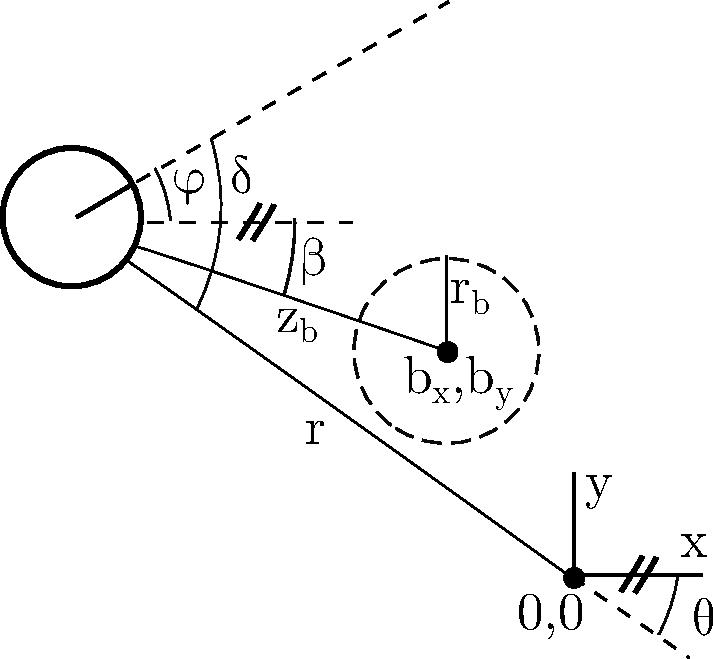
\includegraphics[scale=0.45]{obs.pdf} 
\caption{Egocentric Polar Unicycle Dynamics with Obstacle\label{fig:obs}} 
\end{center}
\end{figure}

A second steering controller is designed to drive the state away from the origin and is defined by the following objective: \begin{equation}z_2=\delta-\text{ atan}(k_1\beta),\label{z2}\end{equation} where $\beta$ is the angle formed between the global positive $x$-axis and the vector $z_b$ pointing from the robot to the obstacle. Figure~\ref{fig:obs} shows the egocentric coordinate system with the addition of the obstacle, where $b_x,b_y$ is the global coordinate of the obstacle and $r_b$ is the minimum safe distance.

The derivative of $z_2$ is similarly computed as with $z_1$, and is given by \begin{equation}\dot{z_2}=\left( 1+\frac{k_1}{1+(k_1\beta)^2}\right) \frac{v}{r}\text{ sin}(z_2+\text{ arctan}(k_1\beta))+\omega.\end{equation} Through feedback linearization of the objective, choosing \begin{equation}\omega = -\frac{v}{r}\left[ k_2 z_2+\left( 1 + \frac{k_1}{1+(k_1\beta)^2} \right) \text{sin}(z_2+\text{ arctan}(-k_1\beta))\right]\end{equation} globally exponentially stabilizes the objective with \begin{equation}\dot{z_2}=-k_2\frac{v}{r}z_2.\end{equation} It is noteworthy that in contrast to the steering objective achieved by $z_1$, the objective of $z_2$ is to make the system unstable with respect to driving the state of the robot to zero; this is done intentionally to allow the robot to navigate around obstacles.

%TODO check the clf stuff
By choosing the angular velocity input $w$ to drive the heading $\delta=\text{ arctan}(-k_1\theta)$, steering control, which drives the state to zero, is achieved. Similarly, choosing the angular velocity input $w$ to drive the heading $\delta=\text{ arctan}(k_1\beta)$ causes the robot to drive away from zero. Thus, there exists a control input that satisfies the control Lyapunov function $\dot{V}<0$; furthermore, following Definition 3 in \cite{ames2014esclf}, the control Lyapunov function is exponentially stabilizing if it satisfies
\begin{equation}
\inf_{u\in U}\left[ \dot{V}+\gamma V \right] \leq 0
\label{eq:esclf}
\end{equation}
for some constant $\gamma >0$, so choosing the correct inputs $u$ will achieve the desired exponential stabilization. According to \cite{amesACC}, by picking a soft constraint relaxation variable $\lambda$, the condition for exponential stabilization shown in \eqref{eq:esclf} is relaxed and can be enforced simultaneously along with a single hard constraint. Because control of the robotic system requires either $\dot{z_1}=-k_2\frac{v}{r}z_1$ or $\dot{z_2}=-k_2\frac{v}{r}z_2$ and $\dot{V}<0$, two soft constrained expressions must be satisfied at a time to achieve exponential stabilization of the state to zero.

\subsection{Hard Constraints as Barrier Functions}
%TODO invariance of C, proof that u satisfy BF
As in \cite{amesACC} and \cite{ames2014esclf}, control barrier functions are a logical way of enforcing safety constraints in navigation from a nonlinear control perspective. 

A zeroing barrier function is used to drive the robot away from obstacles if it leaves the safe set (e.g. the robot gets within an unsafe threshold distance of the obstacle). The safe set $C$ is described by the following expressions:
\begin{align}
C &= {x \in \mathbb{R}^3 | z_b\geq z_{safe}}\\
\partial C &= {x \in \mathbb{R}^3 | z_b=z_{safe}}\\
\text{Int}(C) &= {x \in \mathbb{R}^3 | z_b > z_{safe}}
\end{align}

As presented in \cite{ames2015robust}, a barrier function is a zeroing barrier function $h(x)$ if $\dot{h}(x)\leq \gamma h(x).$ For the purpose of avoiding obstacles in the event that the robot leaves the safe set, a zeroing barrier function was chosen with the following form:
\begin{equation}
h(x)=\sqrt{(-v\text{ cos}(\theta)-b_x)^2+(v\text{ sin}(\theta)-b_y)^2}.
\end{equation}
The derivative of $h(x)$ is given by the following expression:
\begin{equation}
\begin{split}
\dot{h}(x)=\frac{1}{h(x)}[(-v\text{ cos}(\delta)(r-b_y\text{ sin}(\theta)+b_x\text{ cos}(\theta)) \\
-v\text{ sin}(\delta)(b_x\text{ sin}(\theta)+b_y\text{ cos}(\theta))]
\end{split}
\label{zbf}
\end{equation}

A barrier function was chosen to prevent the robot from leaving the safe set. According to Definition 2 in \cite{amesACC}, the barrier function $B$ is a control barrier function if 
\begin{equation}
\inf_{u\in U}\left[ \dot{B}+\frac{\gamma}{B} \right] \leq 0.
\label{eq:cbf}
\end{equation} Thus, by satisfying the equation $\dot{B}\leq 1/B$, the barrier function will prevent the robot from leaving the safe set. The barrier function was chosen to be
\begin{equation}
B=\frac{1}{h(x)-z_{safe}},
\label{bf}
\end{equation}
and its derivative is given by
\begin{equation}
\dot{B}=\frac{-\dot{h}(x)}{(h(x)-z_{safe})^2}.
\end{equation}

%TODO check constraints
\subsection{QP Based Controller}
Quadratic programming is used to find control inputs that simultaneously satisfy both the soft and hard constraints of the system. To minimize control inputs, the cost function $\textbf{u}^TH\textbf{u}+F^T\textbf{u}$ is chosen. The QP is given by the following expression:
\begin{equation}
u^*(x,z) = \argmin_{\textbf{u}=
\left[\begin{matrix}
v\\
\omega\\
\lambda_1\\
\lambda_2\\
\alpha_1\\
\alpha_2
\end{matrix}\right]
\in \mathbb{R}^6}
\frac{1}{2}\textbf{u}^TH\textbf{u}+F^T\textbf{u} 
\label{QP}
\end{equation}
\begin{align}
\text{ s.t.\hspace{1cm}}
\dot{V_1} -\alpha_1 V_1 & \leq\lambda_1\\
\dot{V_2} -\alpha_2 V_2 & \leq\lambda_2\\
\dot{h(x)}-\alpha h(x) & \leq \lambda_1\\
\dot{B} & \leq 1/B\\
0 \leq v & \leq 2.0\\
-0.1\leq \omega & \leq 0.1\\
\alpha_1,\alpha_2 & \leq 0
\end{align}

In \eqref{QP}, the matrix $H\in \mathbb{R}^{6\times 6}$ has the form

\begin{equation}
H=\left[ \begin{matrix}
1 & 0 &0&0& 0 & 0\\
0 &1& 0 &0& 0& 0\\
0& 0 &1& 0& 0& 0\\
0& 0& 0& 1& 0& 0\\
0& 0& 0& 0& 0& 0\\
0& 0& 0& 0& 0& 0\\
\end{matrix}\right],
\end{equation}
and the vector $F^T\in \mathbb{R}^{1\times 6}$ has the form 
\begin{equation}
F^T=\left[ \begin{matrix}
0 & 0 &0&0& 10 & 1\\
\end{matrix}\right].
\end{equation} The last two elements in the diagonal of $H$ were chosen to be zero to ensure that the negative quadratic cost of the slack variables $\alpha_1$ and $\alpha_2$ is as large as possible. Conversely, the last two elements of $F^T$ were chosen to ensure that $\alpha_1$ and $\alpha_2$ were negative to minimize the cost.

The control Lyapunov functions $V_1$ and $V_2$ are the Lyapunov functions correspond to the objectives of driving the state to zero and enforcing the steering control respectively; the equations are given by 
\begin{equation}
V_1=\frac{1}{2}(r^2+\theta^2)
\end{equation} and
\begin{equation}
V_2=\frac{1}{2}z_*^2.
\end{equation}
$z_*$ in $V_2$ represents the different steering objectives $z_1$ and $z_2$ in \eqref{z1} and \eqref{z2}. Because there are two steering objectives, two QP control laws are required: one which drives the state towards the target while avoiding obstacles, and the other that drives the state in such a way that the robot steers away from obstacles. Toggling between steering objectives is dependent on the obstacle measurement. If the measurement of the distance between the robot and the obstacle was less than the minimum safe distance, then the steering objective $z_2$ is used. Otherwise, $z_1$ is used, and $\alpha_1=0$ is additionally enforced. $h(x)$ and $B$ in the QP controller are given in equations \eqref{zbf} and \eqref{bf}. 

\section{Results}
%TODO double check my claims
To test the ability of the QP controller to drive the robot to a target position while simultaneously avoiding obstacles, both simulation and physical experiments were conducted. Simulation results were generated in both MATLAB and Gazebo, and physical results were generated using the robotic platform Jeeves. 

\subsection{Simulation Results}
Two distinct MATLAB simulations were used to validate and test the QP navigation controller. In the first simulation, the controller demonstrates successful navigation of the robot to the target position with and without the presence of obstacles; plots of the state are shown, and the Lyapunov function and its derivative are tracked numerically. In the second simulation, a probabilistic roadmap was used to generate a target trajectory through a map, and the QP navigation controller was applied to drive the robot to the target trajectory while simultaneously avoiding obstacles. 

%TODO add gazebo
Gazebo simulation of a unicycle robot navigating via the QP controller was used to demonstrate the feasibility of the controller in practice.
\subsubsection{Target Position}
Figure~\ref{fig:octoplotsans} shows the output of the first simulation. The navigation objective was to drive the robot from the starting position and heading to zero at the origin. The robot was initialized from eight starting locations, shown in red, with random egocentric headings. The blue lines show the trajectory of the robot, and as expected, the QP controller successfully accomplishes the navigation objective.

\begin{figure}[h!]
\centering
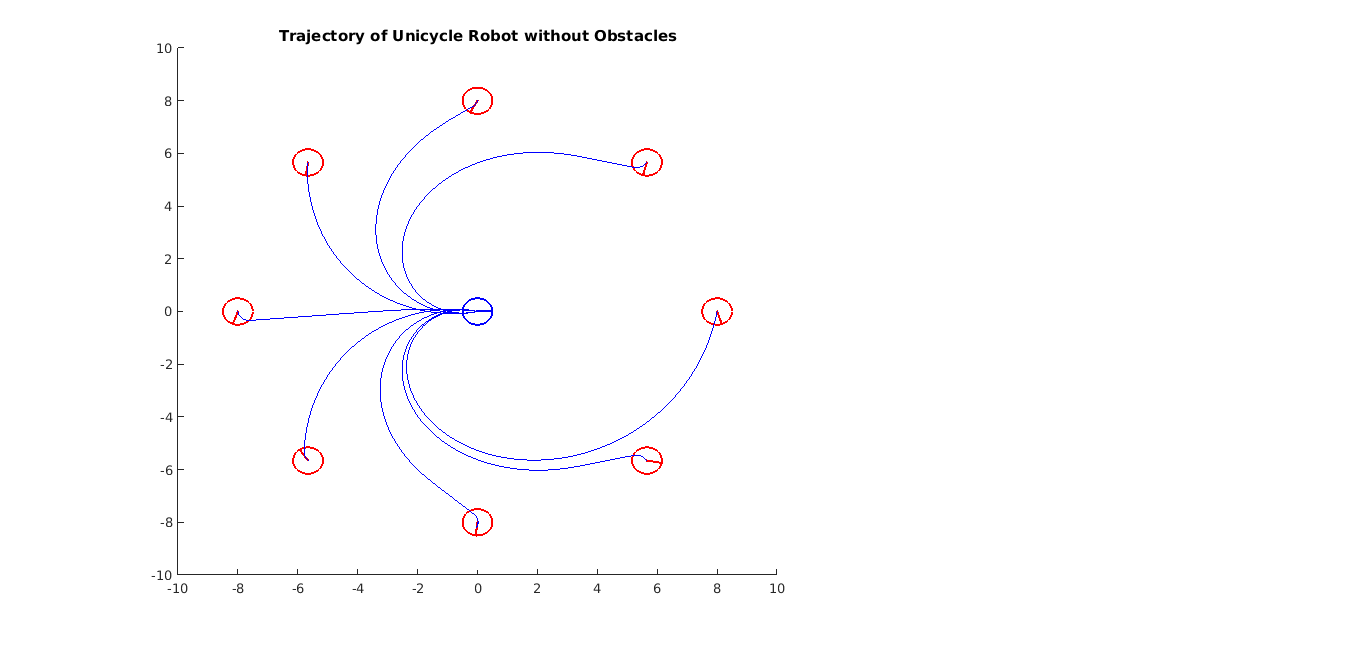
\includegraphics[scale=0.4]{octoPlotCrisisSQR.png} 
\caption{Robot Trajectory in the Absense of Obstacles\label{fig:octoplotsans}} 
\end{figure}

To further evaluate the QP controller and substantiate its success, the state is plotted. Figures~\ref{fig:state} shows that the distance to the target position, the angle $\theta$, and the egocentric heading are successfully zeroed under the QP navigation control protocol.

\begin{figure*}[t]
\centering
\begin{subfigure}[t]{0.32\textwidth}
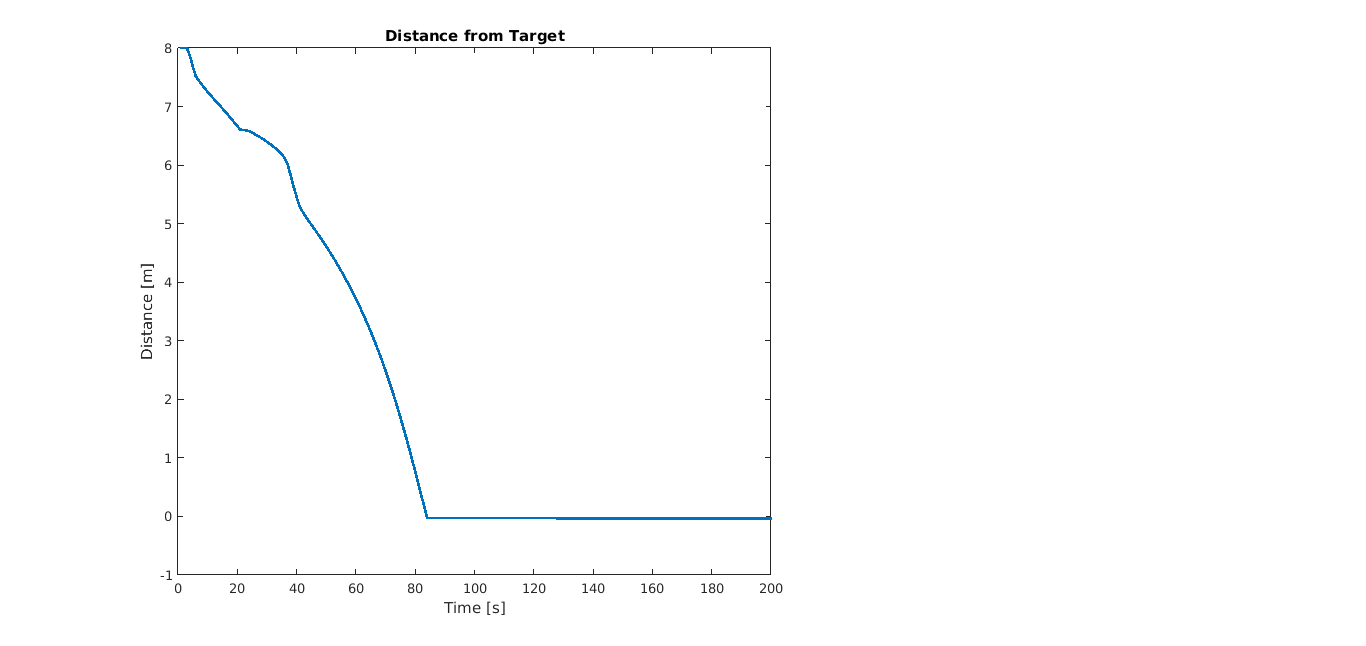
\includegraphics[scale=0.27]{distancetogo.png} 
\caption{Distance of Robot to Target: $r$\label{fig:r}} 
\end{subfigure}
\begin{subfigure}[t]{0.32\textwidth}
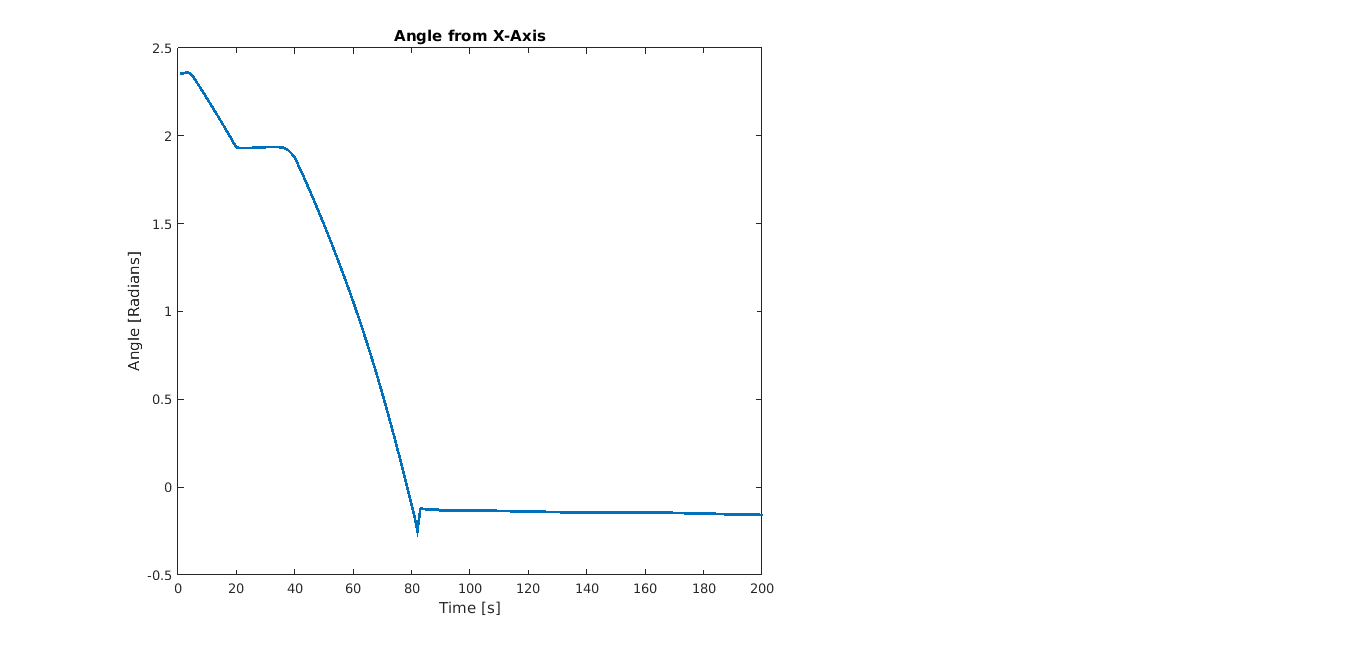
\includegraphics[scale=0.27]{theta.png} 
\caption{Angle between Positive $x$-axis and $r$: $\theta$\label{fig:theta}} 
\end{subfigure}
\begin{subfigure}[t]{0.32\textwidth}
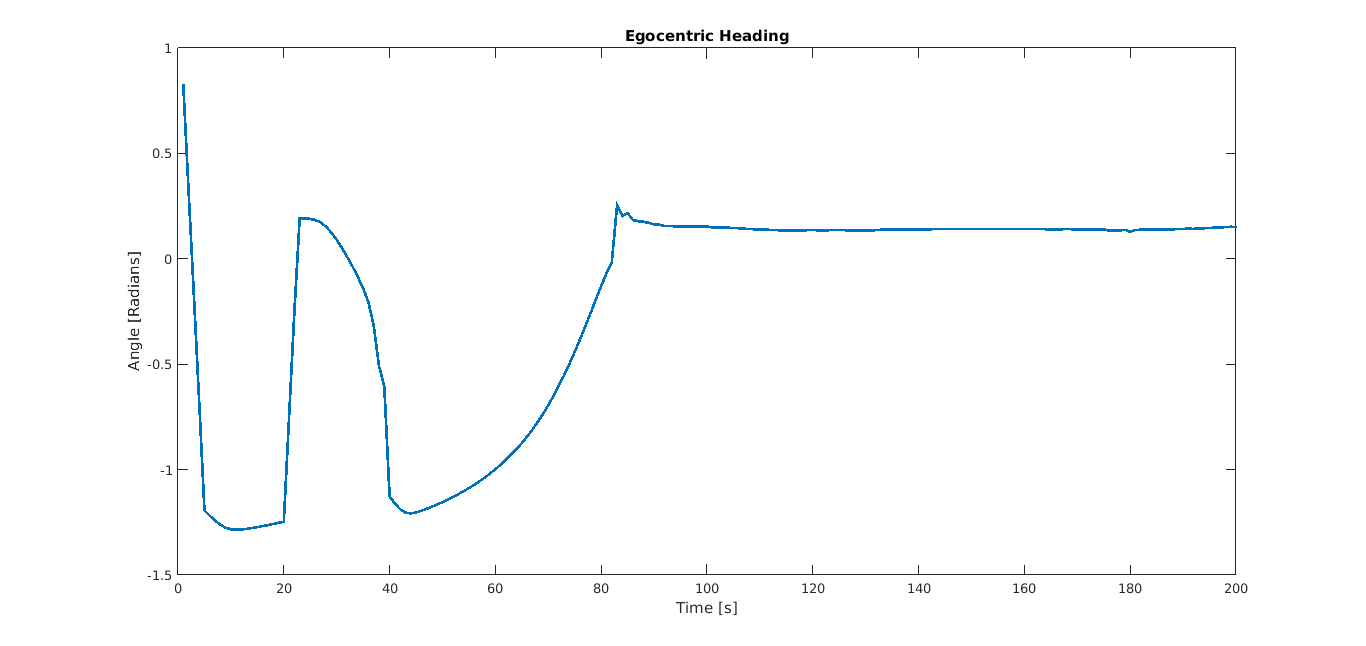
\includegraphics[scale=0.27]{delta.png} 
\caption{Egocentric Heading of Robot: $\delta$\label{fig:delta}} 
\end{subfigure}
\caption{Robot State under QP Navigation Protocol\label{fig:state}}
\end{figure*}

To test the ability of the QP navigation control protocol to prevent collision of the robot with obstacles, robots were again initialized from eight starting positions with random headings, but an obstacle was placed in each robot's path. As Figure~\ref{fig:octoplot} demonstrates, the QP navigation controller simultaneously prevented collision while driving the robot to the desired state.

\begin{figure}[h!]
\centering
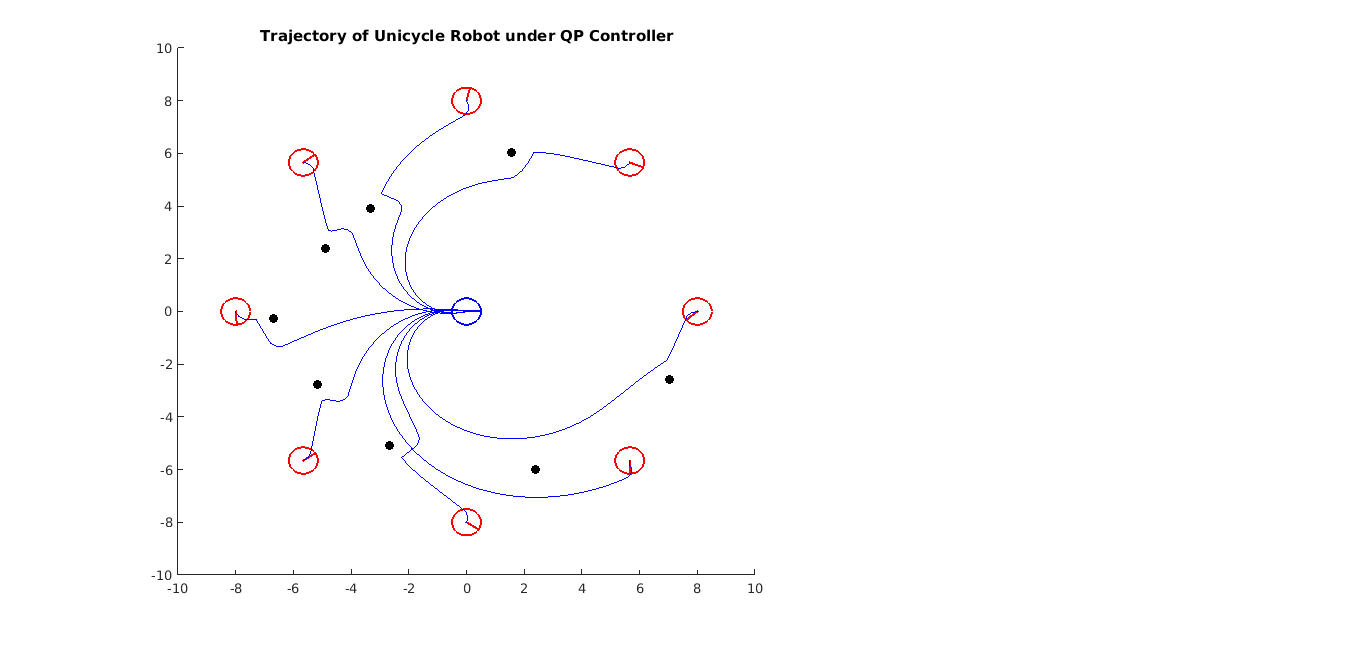
\includegraphics[scale=0.4]{octoPlotProofEditSqur.png} 
\caption{Robot Trajectory in the Presense of Obstacles\label{fig:octoplot}} 
\end{figure}

To numerically validate the relaxed control Lypanuov function in the QP, the value of the Lyapunov function and its derivative were plotted as the robot navigated. For the situation in which obstacles are absent, Figure~\ref{fig:lyapunovsans} shows that the Lyapunov function correctly decays to zero while its derivative remains strictly less than zero until the robot reaches its final destination. With obstacles present, Figure~\ref{fig:lyapunov} ...

\begin{figure}[h!]
\centering
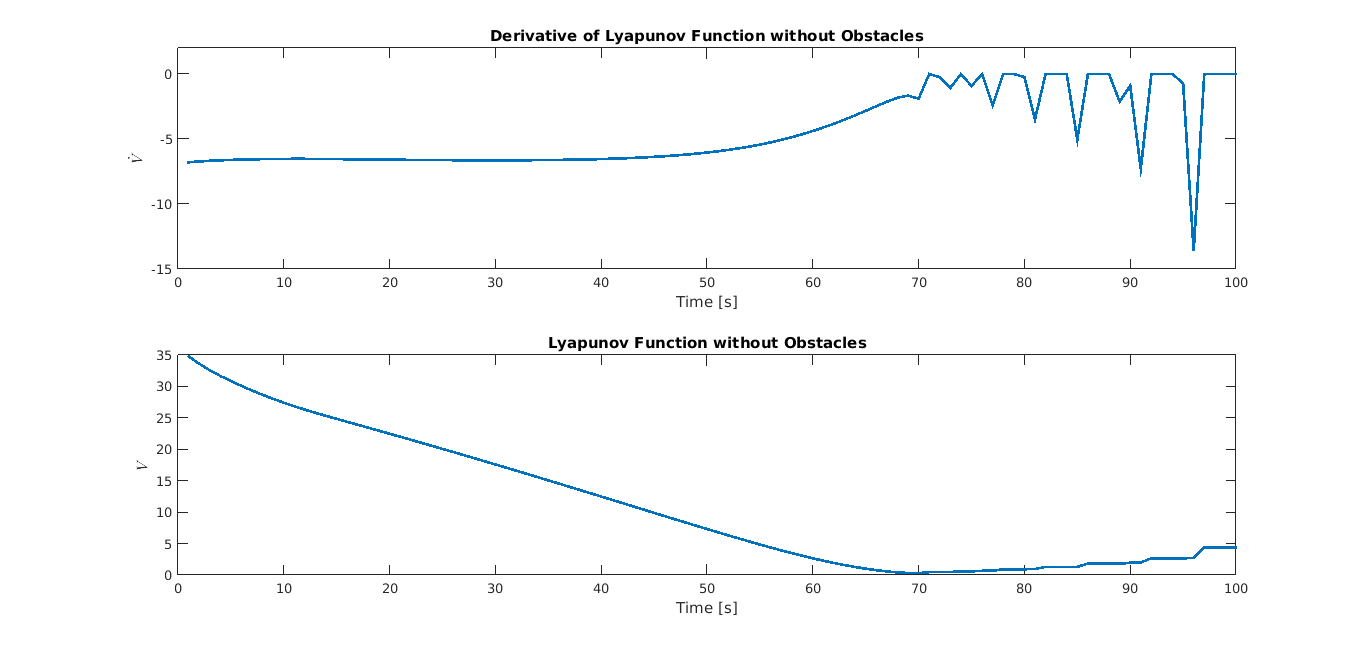
\includegraphics[scale=0.4]{lyapunovsans.png} 
\caption{Lyapunov Function without Obstacles\label{fig:lyapunovsans}} 
\end{figure}

\begin{figure}[h!]
\centering
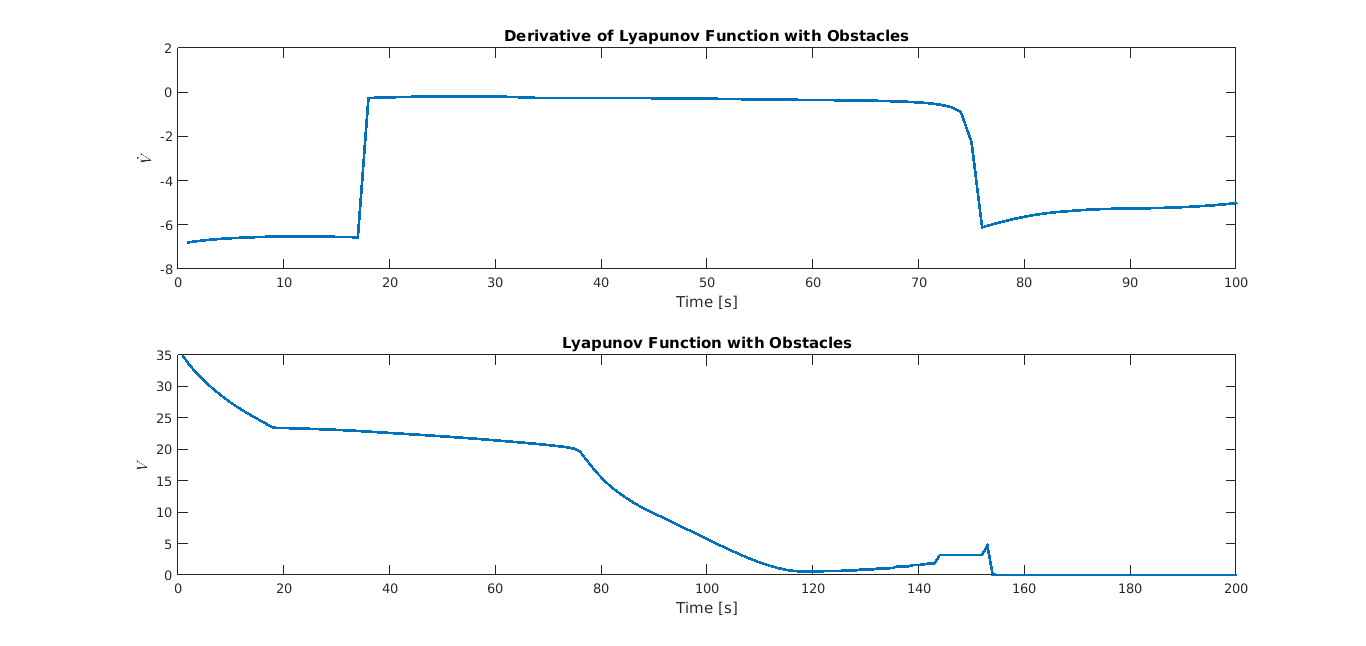
\includegraphics[scale=0.4]{lyapunov.png} 
\caption{Lyapunov Function with Obstacles\label{fig:lyapunov}} 
\end{figure}
 
\subsubsection{Target Trajectory}
\subsubsection{Gazebo}

\subsection{Experimental Results}
\section{Conclusion}

\bibliographystyle{IEEEtran}
\bibliography{IEEEabrv,bibi}

\end{document}